\chapter{Introduction}

\section{Course Information (Winter 2017)}

\begin{itemize}
  \item Instructor: Rosina Kharal
  \item Classroom: RCH 305, Section 001, 8:30\,AM--9:50\,AM
  \item Midterm: February 8, 2017. Final exam: TBA.
\end{itemize}

\paragraph{Recommended texts.}
\begin{enumerate}
  \item Patterson and Hennessy, \emph{Computer Organization \& Design: The
    Hardware/Software Interface}, 5th edition, Morgan Kaufmann, 2013
    (ISBN 0124077269).
  \item (Optional) Harris and Harris, \emph{Digital Design \& Computer
    Architecture}, 2nd edition, Morgan Kaufmann, 2012 (ISBN 0123944244).
\end{enumerate}

\section{Course Outline}

\begin{enumerate}
  \item MIPS basic introduction (five instructions)
  \item Digital logic design
  \item Data representation and manipulation
  \item Designing a datapath
  \item Single-cycle datapath and multi-cycle datapath
  \item Pipelined datapath and pipeline hazards
  \item Memory hierarchies (caches and virtual memory)
  \item ARM: 32-bit (and a look at ARMv8)
\end{enumerate}

\begin{important}[Exam note]
A major part of the final exam covers the last part of the course
(pipelining, memory hierarchy, ARM), so do not neglect it.
\end{important}

\section{Gist of the Course}

This is a \emph{processor} course: it is about how to build a processor and
how it works. We start from the language the processor speaks (its
\emph{instruction set}), build the hardware building blocks from logic
gates, and then assemble those blocks into a working datapath that executes
the instructions. Finally we look at the techniques that make real processors
fast: pipelining and the memory hierarchy.

\section{Instruction Set Architecture}

We write programs in many high-level languages (C, C++, Racket, \ldots), but
the processor understands only one language, a low-level \emph{machine
language}. A compiler translates high-level code to assembly, and an
assembler translates assembly into binary machine code.

\begin{definition}
An \textbf{instruction} is a single operation the processor knows how to
perform, for example \code{add}, \code{sub}, a branch or a jump. The
\textbf{instruction set architecture (ISA)} is the complete set of
instructions, registers, data types and memory model that the hardware
exposes to software. It is the contract between hardware and software.
\end{definition}

The ISA is an abstraction: two processors can implement the same ISA very
differently (one simple and slow, one pipelined and fast) and still run the
same binary programs.

\section{The Big Picture}

Hardware is designed according to a few recurring principles (simplicity
favours regularity, smaller is faster, make the common case fast, good design
demands good compromises). Every computer, from a phone to a server, has the
same five classic components:

\begin{figure}[H]
  \centering
  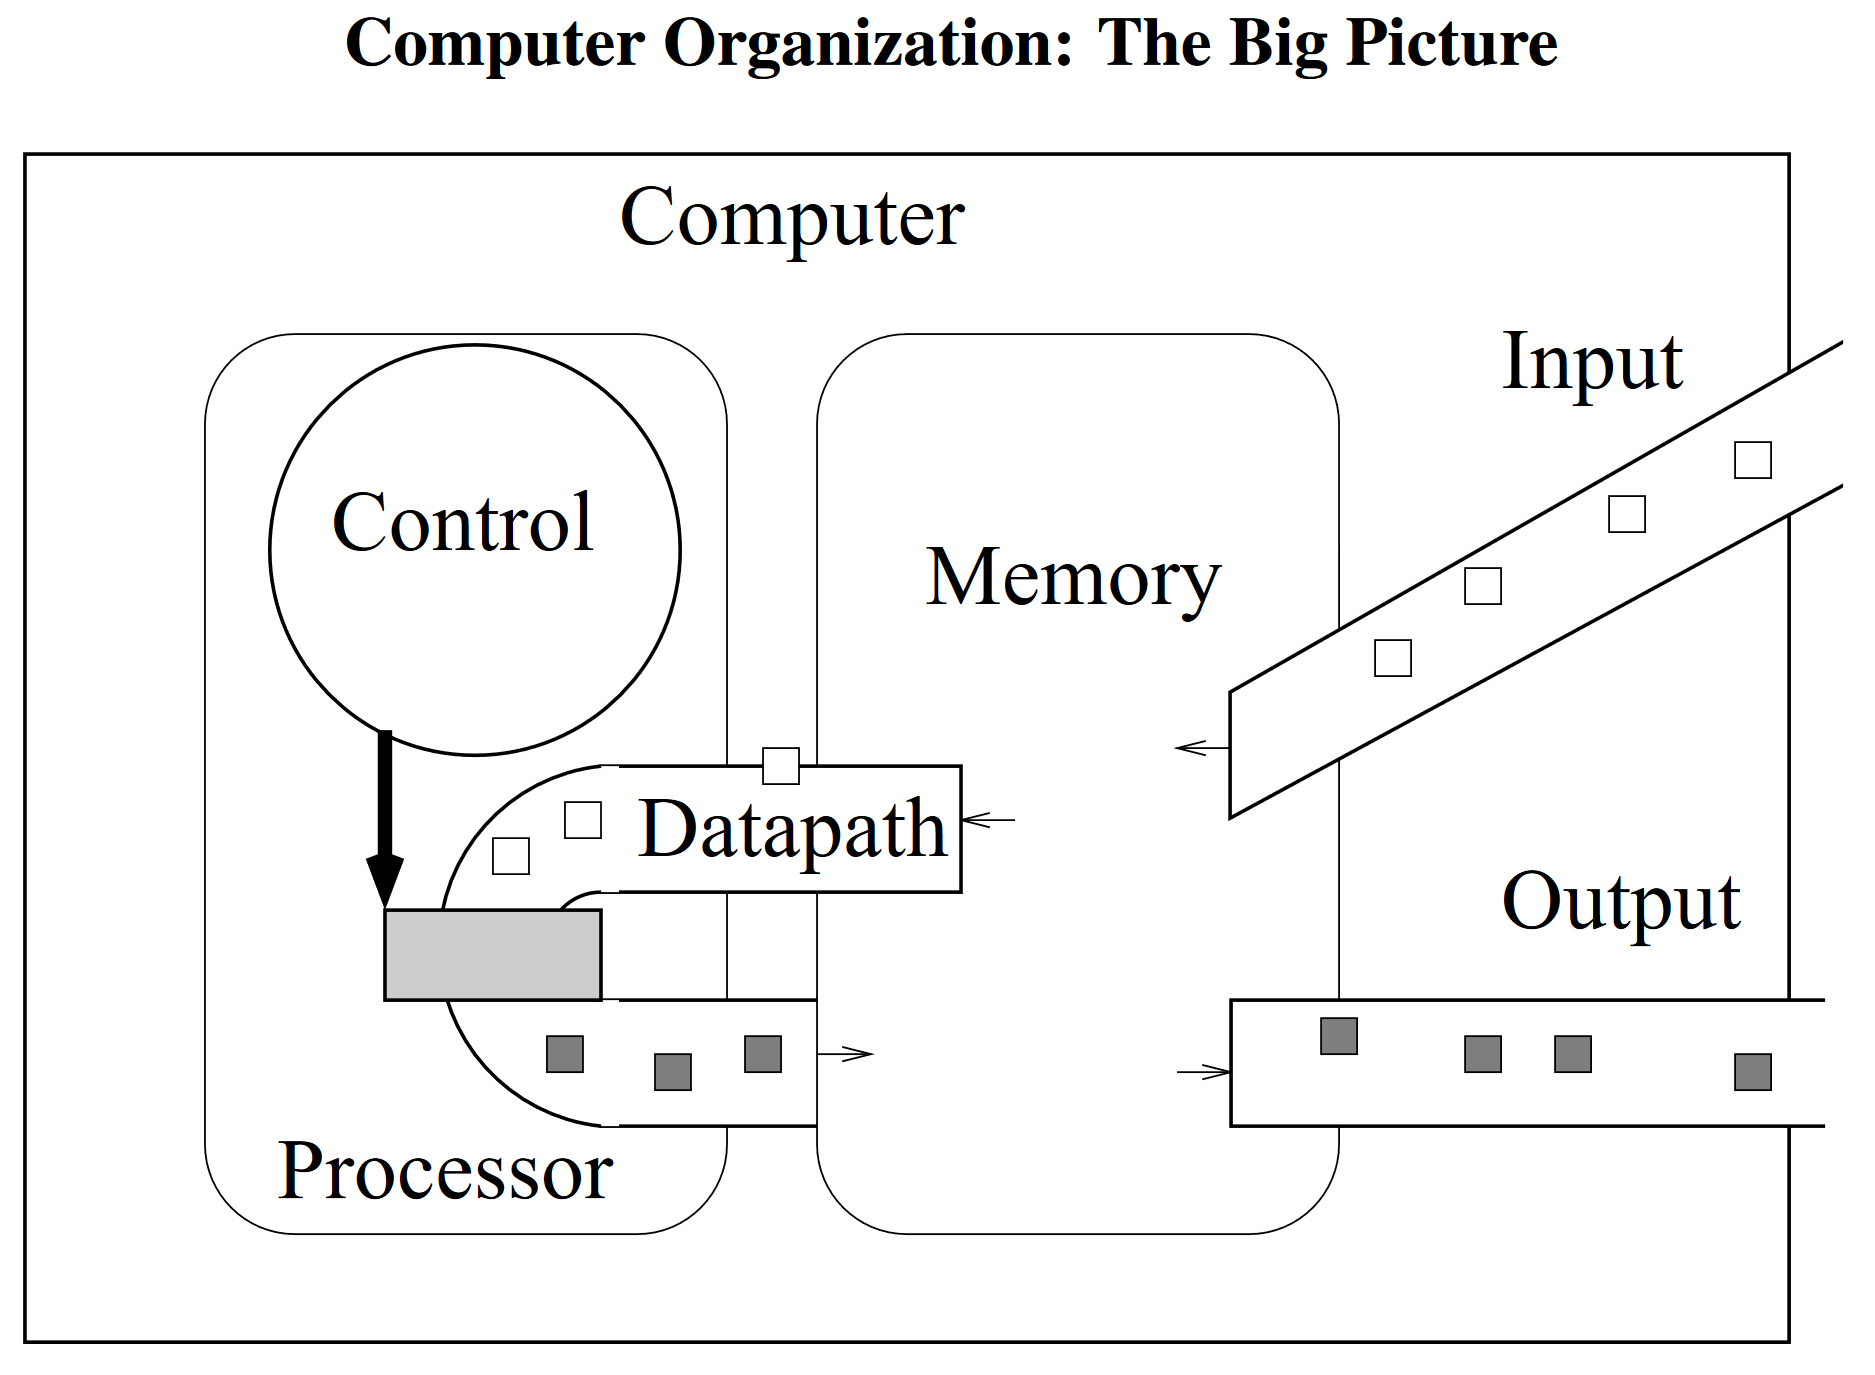
\includegraphics[width=0.75\textwidth]{figures/big-picture.png}
  \caption{The five classic components of a computer: control and datapath
  (together the processor), memory, input and output.}
\end{figure}

\begin{itemize}
  \item \textbf{Datapath}: the hardware that actually performs operations on
    data (registers, ALU, multiplexers, buses). Formally, the datapath is
    the collection of hardware units that come together to execute an
    instruction.
  \item \textbf{Control}: tells the datapath, memory and I/O what to do
    according to the current instruction.
  \item \textbf{Memory}: holds both programs (instructions) and data while
    they are in use (stored-program concept).
  \item \textbf{Input} and \textbf{Output}: devices that bring data in and
    send results out.
\end{itemize}

\section{Assembly Language and MIPS}

Assembly language is a human-readable form of machine code. Each line
corresponds (essentially) to one machine instruction. Different operations
have different names (mnemonics) and different \emph{formats}.

\begin{definition}
\textbf{MIPS} (originally ``Microprocessor without Interlocked Pipeline
Stages'') is a \textbf{RISC} (Reduced Instruction Set Computer) architecture:
\begin{enumerate}
  \item it provides only very basic operations, each doing a small amount of
    work;
  \item all instructions are the same size: in this course, a 32-bit word
    (64-bit versions of MIPS exist but we use the 32-bit one);
  \item the first six bits of every instruction are the \textbf{opcode}.
\end{enumerate}
\end{definition}

The execution of an instruction in hardware is divided into five steps:
instruction fetch, instruction decode/register read, execute (ALU), memory
access, and register write-back. This five-way split will reappear when we
pipeline the processor.

\subsection{Registers}

\begin{definition}
A \textbf{register} is a small, very fast storage location inside the
processor. It plays a role similar to a temporary variable in a high-level
language. MIPS has 32 general-purpose registers, each 32 bits wide.
\end{definition}

\begin{example}
Compile \lstinline[style=c]|f = (g + h) - (i + j);| where the variables
$f, g, h, i, j$ live in registers \code{\$s1}, \ldots, \code{\$s5}:

\begin{lstlisting}[style=mips]
add $t0, $s2, $s3    # t0 = g + h
add $t1, $s4, $s5    # t1 = i + j
sub $s1, $t0, $t1    # f  = t0 - t1
\end{lstlisting}
Since an instruction has only two source operands, we need temporaries
(\code{\$t0}, \code{\$t1}) to hold intermediate results.
\end{example}

Two issues already show up in this tiny example:
\begin{itemize}
  \item \textbf{Data dependency}: the \code{sub} needs the results of both
    \code{add}s, so it cannot run before them. This matters a lot once
    instructions overlap in a pipeline.
  \item \textbf{Overflow}: a 32-bit register cannot hold every sum; adding
    two large numbers may produce a result that does not fit.
\end{itemize}

\subsection{Instruction addresses}

Instructions are stored in memory one after the other. Since every MIPS
instruction is 4 bytes, consecutive instructions are at addresses
$0, 4, 8, 12, \ldots$:

\begin{center}
\begin{tabular}{rl}
\toprule
Address & Instruction \\
\midrule
0  & \code{add \$3, \$2, \$1} \\
4  & \code{sub \ldots} \\
8  & \code{sub \ldots} \\
12 & \code{sub \ldots} \\
\bottomrule
\end{tabular}
\end{center}

\subsection{The three MIPS instruction formats}

The \emph{format} of an instruction describes how many operands it has and
of what type.
\begin{itemize}
  \item \textbf{R-format} (register): \code{add \$1, \$2, \$3} adds the
    contents of \code{\$2} and \code{\$3} and stores the result in
    \code{\$1}. Often written \code{add rd, rs, rt} where \code{rd} is the
    destination register.
  \item \textbf{I-format} (immediate): \code{addi \$1, \$2, 100} adds the
    constant 100 to \code{\$2} and stores the result in \code{\$1}.
  \item \textbf{J-format} (jump): \code{j 28}, used for unconditional
    jumps (details later).
\end{itemize}

\subsection{Jumping counts words, not bytes}

When we say ``jump to instruction 40'' we mean the 40th instruction (word),
so the program counter moves to byte address $40 \times 4 = 160$. Because
every instruction is 4 bytes, the low two bits of an instruction address are
always $00$, and MIPS saves encoding space by storing word offsets and
multiplying by 4 in hardware.

\section*{Summary}
\begin{itemize}
  \item CS 251 is about how a processor is built: ISA, digital logic,
    datapath and control, pipelining, memory hierarchy.
  \item The ISA is the hardware/software contract; MIPS is a simple 32-bit
    RISC ISA with fixed-length instructions and a 6-bit opcode.
  \item A computer = datapath + control (processor) + memory + input + output.
  \item Registers are fast local storage; MIPS has 32 of them.
  \item Three formats: R (three registers), I (two registers + constant),
    J (jump target). Instruction addresses go up by 4.
\end{itemize}
